%15 min preso!
\documentclass[xcolor=table,aspectratio=169]{beamer}
\usepackage{beamerthemesplit}
\usepackage{wrapfig}
\usetheme{SPbGU}
\usepackage{pdfpages}
\usepackage{amsmath}
\usepackage{cmap}
\usepackage[T2A]{fontenc}
\usepackage[utf8]{inputenc}
\usepackage[english]{babel}
\usepackage{indentfirst}
\usepackage{amsmath}
\usepackage{tikz}
\usepackage{multirow}
\usepackage[noend]{algpseudocode}
\usepackage{algorithm}
\usepackage{algorithmicx}
\usepackage{fancyvrb}
\usepackage{hyperref} 
\usetikzlibrary{calc}
\usetikzlibrary{shapes, backgrounds}
\usetikzlibrary{arrows,automata}
\usetikzlibrary{positioning}
\usetikzlibrary{fit}
\usetikzlibrary{shapes.callouts}
\usetikzlibrary{shapes.misc}
\usepackage{xparse}
\usepackage{fontawesome}

\usepackage{etoolbox,refcount}
\usepackage{multicol}

\usepackage{tabularx}
\newcolumntype{Y}{>{\raggedleft\arraybackslash}X}

\renewcommand{\thealgorithm}{}

\newtheorem{mytheorem}{Theorem}
\renewcommand{\thealgorithm}{}

\newcommand{\tikzmark}[1]{\tikz[overlay,remember picture] \node (#1) {};}
\def\Put(#1,#2)#3{\leavevmode\makebox(0,0){\put(#1,#2){#3}}}

\newcommand{\ltz}{$< 1$}

\tikzset{
    state/.style={
           rectangle,
           rounded corners,
           draw=black, very thick,
           minimum height=2em,
           inner sep=2pt,
           text centered,
           },
}

\tikzset{
    invisible/.style={opacity=0,text opacity=0},
    visible on/.style={alt=#1{}{invisible}},
    alt/.code args={<#1>#2#3}{%
      \alt<#1>{\pgfkeysalso{#2}}{\pgfkeysalso{#3}} % \pgfkeysalso doesn't change the path
    },
}

\tikzset{cross/.style={cross out, draw=black, minimum size=2*(#1-\pgflinewidth), inner sep=0pt, outer sep=0pt, ultra thick},
%default radius will be 1pt. 
cross/.default={1pt}}

\NewDocumentCommand{\mycallout}{r<> O{opacity=0.8,text opacity=1} m m m}{%
\tikz[remember picture, overlay]\node[align=center, fill=cyan!20, text width=#5cm,
#2,visible on=<#1>, rounded corners,
draw,rectangle callout,anchor=pointer,callout relative pointer={(290:0.5cm)}]
at (#3) {#4};
}

\NewDocumentCommand{\mycalloutR}{r<> O{opacity=0.8,text opacity=1} m m m}{%
\tikz[remember picture, overlay]\node[align=center, fill=cyan!20, text width=#5cm,
#2,visible on=<#1>, rounded corners,
draw,rectangle callout,anchor=pointer,callout relative pointer={(30:0.8cm)}]
at (#3) {#4};
}


%callout relative pointer={(230:0.5cm)}]

\newcounter{countitems}
\newcounter{nextitemizecount}
\newcommand{\setupcountitems}{%
  \stepcounter{nextitemizecount}%
  \setcounter{countitems}{0}%
  \preto\item{\stepcounter{countitems}}%
}
\makeatletter
\newcommand{\computecountitems}{%
  \edef\@currentlabel{\number\c@countitems}%
  \label{countitems@\number\numexpr\value{nextitemizecount}-1\relax}%
}
\newcommand{\nextitemizecount}{%
  \getrefnumber{countitems@\number\c@nextitemizecount}%
}
\newcommand{\previtemizecount}{%
  \getrefnumber{countitems@\number\numexpr\value{nextitemizecount}-1\relax}%
}
\makeatother    
\newenvironment{AutoMultiColItemize}{%
\ifnumcomp{\nextitemizecount}{>}{3}{\begin{multicols}{2}}{}%
\setupcountitems\begin{itemize}}%
{\end{itemize}%
\unskip\computecountitems\ifnumcomp{\previtemizecount}{>}{3}{\end{multicols}}{}}


\beamertemplatenavigationsymbolsempty

\title[High-performance graph analysis]{High-Performance Graph Analysis}
\institute[SPbSU]{
Saint Petersburg State University
}

% То, что в квадратных скобках, отображается в левом нижнем углу.
\author[Semyon Grigorev]{Semyon Grigorev}

\date{March 22, 2024}


%Я предлагаю сначала в общем рассказать интересы и компетенции группы, 
%что научная группа сделала за 3 месяца, 
%потом потратить 1 страницу презентации на каждого из студентов (что сделал, почему важно для Yiming, какие планы). 
%В конце перейти к планам на год.

\begin{document}
{
\begin{frame}[fragile]
  \begin{table}
  \centering
  %
\includegraphics[height=1.5cm]{pictures/SPbGU_Logo.png}
  \begin{tabularx}{\linewidth}{XcX}
    %
\includegraphics[height=0.9cm]{pictures/hu_logo.jpeg} 
    \hfill
    & 
    & \hfill 
\includegraphics[height=1.6cm]{pictures/SPbGU_Logo.png}
  \end{tabularx}
  \end{table}
  \titlepage
\end{frame}
}

\begin{frame}[fragile]
  \frametitle{Research Landscape}
  \begin{minipage}{0.55\textwidth}
    \begin{itemize}
      \item Formal language constrained path querying\footnote{For given language $\mathcal{L}$ and edge-labelled graph $\mathcal{G}$ find $R=\{ \pi \mid \pi \text{ --- path in }\mathcal{G}, \omega(\pi) \in \mathcal{L}\}$,
      $\omega(v_0 \xrightarrow{l_0} v_1 \xrightarrow{l_1} v_2 \ldots) = l_0 l_1 \ldots$} 
      \begin{itemize}
        \item Regular path querying (RPQ): partially supported in OpenCypher, part of GQL
        \item Context-free path querying (CFPQ, CFL-r): proposal to OpenCypher
      \end{itemize} 
      \item Linear algebra based graph analysis
      \begin{itemize}
        \item Specialized libraries for linear algebra (including GPGPU)
        \item Specialized optimizations
        \item New linear algebra based algorithms
      \end{itemize}
    \end{itemize} 
  \end{minipage}~  
  \begin{minipage}{0.4\textwidth}
    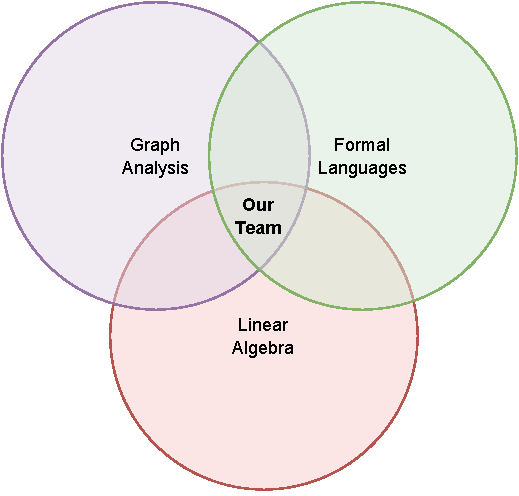
\includegraphics[width = 0.9\textwidth]{pictures/ResearchArea.drawio.pdf}
  \end{minipage}
\end{frame}

\begin{frame}[fragile]
  \frametitle{Context-Free Path Querying (CFPQ)}
  \begin{itemize}
    \item Multiple source CFPQ for RedisGraph
    \begin{itemize}
      \item The \textbf{first full-stack CFPQ support}: OpenCypher and execution plan extension, evaluation algorithm
    \end{itemize}
    \item CFPQ for Neo4j
      \begin{itemize}
        \item GLL-based (non-matrix) CFPQ algorithm 
        \item \textbf{Computes all paths}, not reachability facts only
      \end{itemize}
    \item Generic CFPQ solver
    \begin{itemize}
      \item \href{https://arxiv.org/abs/2401.11029}{Optimization of the Context-Free Language Reachability Matrix-Based Algorithm}
      \item \textbf{Outperforms state-of-the-art generic CFPQ solvers and some specialized solutions}
    \end{itemize}
  \end{itemize}
\end{frame}


\begin{frame}[fragile]
  \frametitle{\faGears \ Regular Path Querying (RPQ)}
  \begin{itemize}
    \item Linear algebra based multiple source RPQ    
    \item Work in progress    
  \end{itemize}
\end{frame}


\begin{frame}[fragile]
  \frametitle{Spla\footnote{\href{https://github.com/SparseLinearAlgebra/spla}{https://github.com/SparseLinearAlgebra/spla}}}
  Generalized sparse linear algebra library with vendor-agnostic GPUs accelerated computations 
  \vfill
  \begin{minipage}{0.48\textwidth}
    \centering
    Performance comparison
    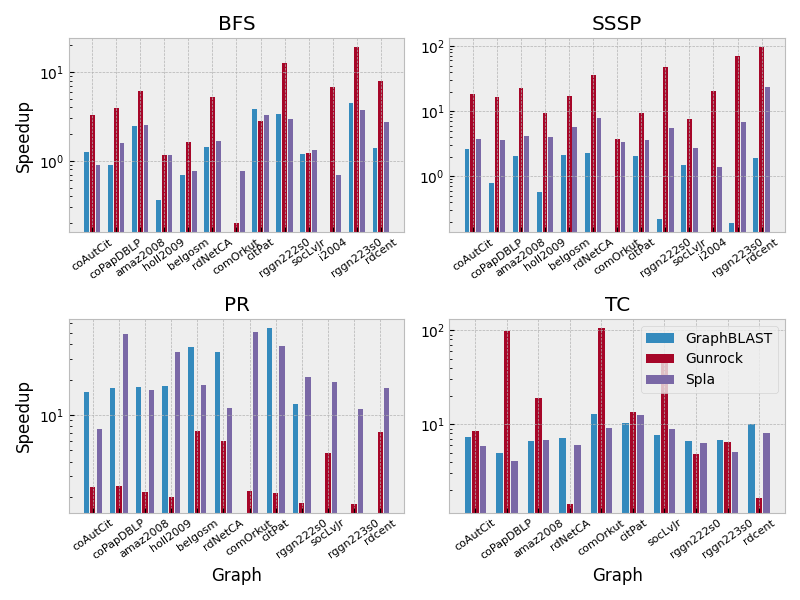
\includegraphics[width = 0.95\textwidth]{pictures/rq1_rel_compact.png}  
  \end{minipage}
  ~
  \begin{minipage}{0.48\textwidth}
    \centering
    Portability
    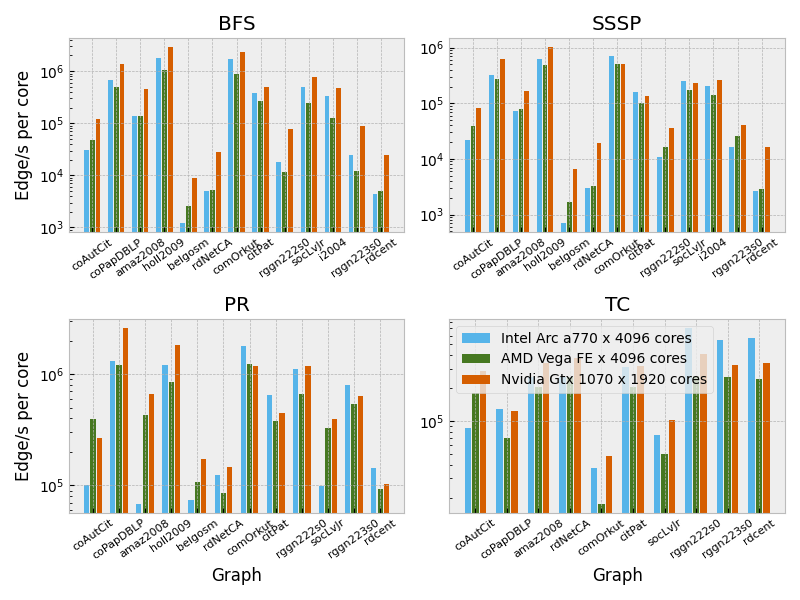
\includegraphics[width = 0.95\textwidth]{pictures/rq2_cores_compact.png}
  \end{minipage}
  
\end{frame}

\begin{frame}[fragile]
  \frametitle{Research Directions}
  \begin{itemize}
    \item Graph analysis algorithms research and development
    \begin{itemize}
      \item CFPQ and RPQ algorithms evaluation, optimization, etc. 
      \item Dataset collection (for CFPQ, RPQ)
      \item New graph algorithms development
    \end{itemize}
    \item Specialized software and hardware for high-performance linear algebra
    \begin{itemize}
      \item Generic sparse linear algebra library with GPGPU support (Spla)
      \item High-level optimizations for linear algebra (kernel fusion)
      \item Specialized hardware for linear algebra: lambda-processors
    \end{itemize}
    
  \end{itemize}
\end{frame}


\end{document}
